% !TeX root = main.tex
% !TeX TS-program = xelatex
\documentclass[AutoFakeBold, songti]{iNSFC}
\usepackage{array}
\usepackage{longtable}
\usepackage{colortbl}
\usepackage{multirow}
\graphicspath{{figs/}}   % 设置图片所存放的目录
\addbibresource{ref.bib}

\begin{document}


%%%%%%%%% TITLE %%%%%%%%%
%\begin{center}
%	{\zihao{3} \textbf{报告正文}  \vspace{-3.8ex}}
%\end{center}  
\qianyan

%%%%%%%%% Your Content %%%%%%%%%
%(一)立项依据与研究内容

\NsfcChapter{(一)立项依据与研究内容}{(建议8000字以内):}

\NsfcSection{项目的立项依据}{(研究意义、国内外研究现状及发展动态分析,需结合科学研究发展趋势来论述科学意义;或结合国民经济和社会发展中迫切需要解决的关键科技问题来论述其应用前景。附主要参考文献目录);}

对于高校教师和研究人员来说,国家自然科学基金(National Natural Science Foundation of China,NSFC)非常重要,写出能让所有专家都满意的本子也相当的耗时。对于平时只采用 LaTeX 格式投稿论文的老师来说,由于基金委只给出了 Word 模板,这种切换大致会有下面一些不方便:
\begin{itemize}
	\item 本子中很可能会用到以往小论文中的公式、图表以及参考文献,无法直接复制粘贴,要将一模一样的内容从 LaTeX 转换成 Word 需要不少时间;
	\item Word 中对参考文献、图表、公式的交叉引用没有 LaTeX 来的方便。
\end{itemize}
很自然的,如果能有一个国家自然基金的 LaTeX 模板就好了,可以挤出更多的时间来关注内容,而非格式以及排列参考文献这种机械无聊的事情上。

\subsection{相关工作}
目前知道的 NSFC 模板一共两个,一个是 NSFC 官方给出的 Word 模板,也是LaTeX 模板的仿制对象。青年基金和面上基金的模板是一模一样的,本文的 LaTeX 模板也只是针对青年和面上,毕竟其他模板还无缘得见。Word 模板的具体样式如下:
\begin{enumerate}[fullwidth,itemindent=0em, label=\arabic*)]
	\item \textbf{页面布局:}
	      \begin{itemize}[itemindent=2em]
	      	\item \textbf{页边距:}上 2.54 厘米;下 2.54 厘米;左 3.2 厘米;右 3.2 厘米;装订线:0 厘米;
	      	\item \textbf{纸张:}A4,宽度 21 厘米,高度 29.7 厘米;
	      	\item \textbf{版式:}距边距 页眉 1.5 厘米,页脚 1.75 厘米。
	      \end{itemize}
	\item \textbf{文字:}
	      \begin{itemize}[itemindent=2em]
	      	\item \textbf{正文标题:}字体是 加粗的楷体二号,段后间距 0.5 行,行距为固定值 22 磅;
	      	\item \textbf{一级大标题:}楷体四号,段后间距 0.5 行,行距为固定值 22 磅;前半部分加粗,后半部分不加粗;
	      	\item \textbf{二级标题:}楷体四号,行距为固定值 22 磅;前部的数字标号不加粗,中部文字加粗,最后部分不加粗;关于段后行距,部分有0.5行,部分没有,Word模板没统一,个人认为统一有更美观一些;
	      	\item \textbf{颜色:}蓝色,RGB 数值为 (0, 112, 192)。
	      \end{itemize}  
\end{enumerate}

另一个模板是2017年1月8号,南开大学的程明明教授\footnote{程明明教授个人主页:\href{http://mmcheng.net}\href{http://mmcheng.net}}曾在 CTeX 论坛上给出过一个国家自然科学基金的 LaTeX 模版\footnote{程明明教授提供的模板:\href{http://www.latexstudio.net/archives/9308}{http://www.latexstudio.net/archives/9308}}。受程明明教授先驱工作的启发,我们也做了一点微小的工作。

\subsection{动机}
已有珠玉在前,我们之所以还要重新造轮子,主要是参考了最新一年青年和面上基金模板,重新修改了页面布局、字体类型和大小以及颜色、标题内容,以期做到与 Word 模板尽可能的相似。主要贡献如下:
\begin{itemize}
	\item 重新设置了页面布局、字体类型和大小以及颜色、标题内容,基本做到了尽可能的相似;
	\item 参考文献完全依照国标 gbt7714-2005,修正了部分 Bug,提供了新的引用命令;
	\item 替换并引入了一些新的宏包,增加了更多的选项,定制性更好。
\end{itemize}
如果说还有一点成绩就是写了这篇啰哩啰唆的文档,对于 LaTeX 新人,也能够比较方便地根据自己的需求修改模板。因为是在程明明教授作品的基础上改进的,为表示尊重,我们把我们的模板叫作 improved NSFC template,简称为 iNSFC。

最新的模板可以从 Github 上的项目主页\footnote{最新模板 Github 地址:\href{https://github.com/YimianDai/iNSFC}{https://github.com/YimianDai/iNSFC}}下载到。为防 Github 惨遭不测,国内用户也可访问 coding.net 上的项目备份\footnote{最新模板 coding.net 地址:\href{https://coding.net/u/YimianDai/p/iNSFC/git}{https://coding.net/u/YimianDai/p/iNSFC/git}}下载最新模板。
匆忙写就,难免疏忽。对于不足之处,欢迎在 Github 提交 issue,在文章留言区留言\footnote{留言区地址:\href{http://lowrank.science/NSFC-LaTeX/}{http://lowrank.science/NSFC-LaTeX/}},或者直接给我写邮件(yimian dot dai at gmail dot com),在此先行谢过各位。

\NsfcSection{项目的研究内容、研究目标,以及拟解决的关键科学问题}{(此部分为重点阐述内容);}

\textbf{最新文档请看 ReadMe,下文只做测试用。}

\subsection{编译}
由于 CTeX 宏集的行为会受编译方式影响,比如不同编译方式下 CTeX 宏集底层的中文支持方式也会不同。LaTeX 和 pdfLaTeX 为 CJK 宏包,XeLaTeX 为 xeCJK 宏包,LuaLaTeX 为 LuaTeX-ja 宏包;使用 XeLaTeX 和 LuaLaTeX 编译时,CTeX 宏集使用 UTF-8 编码,LaTeX 和 pdfLaTeX 时使用 GBK 编码。最终的排版效果因不同编译方式而已。

\textbf{本模板唯一推荐使用的是 XeLaTeX},可以获得与 Word 模板最接近的效果。发行版为 TeXLive 2015 或者 2016 均可,但在 TeXLive 2014 中编译会不通过,因为 CTeX 在 14 和 15 之间有了重大更新。这里暂不推荐其他发行版,毕竟按照 CTeX 套装开发者 L 叔\footnote{L 叔主页:\href{http://liam0205.me/}{http://liam0205.me/}}的名言
\begin{quote}
	选择 TeX Live,选择简单的人生;\\
	选择 MiKTeX,选择麻烦的人生;\\
	选择 CTeX 套装,选择崩溃的人生。
\end{quote}

demo.tex 用 LuaLaTeX 也可以编译通过,但标题加粗部分会不再是粗体;如果想使用 pdfLaTeX,需要在 insfc.sty 中将\textbackslash usepackage\{fontspec\} 注释掉,NsfcChapter 和 NsfcSection 命令中的 \textbackslash setmainfont\{KaiTi\} 去掉,但标题中的数字字体将不再是楷体,而且字宽会变宽一点。为了能够让 Sublime Text 中的 LaTeXTools 这样的插件也可以顺利编译,在 demo.tex 中也需要将第一行注释的 xelatex 改为对应的 lualatex 或者 pdflatex。

经过 chengsshi 测试,将 .tex 中第三行的 linespread=1.56 去掉 CTeX 套装也能够编译通过,但注意请将编译结果与模板中给出的 PDF 对比一下。

\subsubsection{Mac 用户}
% 如果是 Mac 版 TeXlive 用户需要更改默认楷书字体,把 insfc.sty 里的 KaiTi 改成 Kai 就能正常编译通过了,但这样做粗体字显示不出来。林智老师告诉我,在 Mac OS 10.12 Sierra 上用 TeXLive 2016 的 xeLaTeX 编译,需要对 insfc.sty 作如下改动,加入
% \begin{minted}[autogobble]{latex}
% 	\setCJKfamilyfont{zhkai}[BoldFont={Kaiti SC Bold}]{Kaiti SC} 
% 	\setCJKfamilyfont{zhsong}[BoldFont={Songti SC Bold}]{Songti SC} 
% \end{minted}
% 因为新版 mac 系统和 ctex 宏包在字体名上有冲突,需要重新命名
% 章名字体 \mintinline{TeX}{\setmainfont{KaiTi}} 需要改为 \mintinline{TeX}{\setmainfont{STKaiti}} (注意大小写)
% 节序号字体 \mintinline{TeX}{\setmainfont{KaiTi}} 改为 \mintinline{TeX}{\setmainfont{STHei}} (Mac 中楷体数字字体都对不上)


\subsection{字体}
就个人审美而言,正文使用楷体比宋体更加美观。所以我们专门设置了楷体,如果用户想要将自己的内容设置为宋体,只需在 .tex 文件中将下列代码注释掉:

% \begin{minted}{latex}
% 	% 导言区中部  
% 	\DeclareCaptionFont{capfont}{\kaishu\zihao{-4}\selectfont} % Caption font
% 	\DeclareCaptionFont{subfont}{\kaishu\zihao{5}\selectfont} % Sub-caption font
% 	\captionsetup{font = capfont}
% 	\captionsetup[subfigure]{font = subfont}
% 	% \begin{document} 下方
% 	\kaishu
% \end{minted}

% \textbf{text}

% \textbf{加粗}

% \textit{text}

% \textit{斜体}

\subsection{参考文献}
在 insfc.sty 中,关于参考文献的设置如下,可以看到,我们使用了 natbib 宏包来定制参考文献,除了常用的 \textbackslash cite\{\} 命令来提供上角标的参考文献引用,如 Bengio 等学者\citess{bengio2013representation} XXXX。还提供了 \textbackslash inlinecite\{\} 命令用于提供行内的引用,如文献\inlinecite{li2014object}提出了XXX。最后一句代码用于调节参考文献条目之间距离。

% \begin{minted}[
% 		frame=lines,
% 		framesep=2mm,
% 		baselinestretch=1.2,
% 		fontsize=\footnotesize,
% 	linenos]{latex}
% 	\usepackage[square,numbers,sort&compress]{natbib}
% 	\newcommand{\citess}[1]{\textsuperscript{\cite{#1}}}
% 	\setlength{\bibsep}{1pt plus 0.3ex}
% \end{minted}

参考文献的字体、大小和样式风格,可以在 .tex 文件中下面代码里调节。gbt7714-nsfc.bst 文件基于南京大学计算机科学与技术系胡海星博士的 GBT7714-2005-BibTeX-Style 项目\footnote{GBT7714-2005-BibTeX-Style 项目:\href{https://github.com/Haixing-Hu/GBT7714-2005-BibTeX-Style}{https://github.com/Haixing-Hu/GBT7714-2005-BibTeX-Style}},我们在此基础上稍做了一点修改,使得英文人名从全部字母大写变为只有首字母大写。

% \begin{minted}{latex}
% 	\begin{spacing}{1.3}  
% 		\zihao{5} \songti   
% 		\bibliographystyle{gbt7714-nsfc}
% 		\bibliography{ref}
% 	\end{spacing}
% \end{minted}

因为写 demo,我把参考文献放这里了,真写本子的时候,还是要放在国内外概况那边。

% 因为写 demo,我把参考文献放这里了,真写本子的时候,还是要放在国内外概况那边
\begin{bibenv}
	\bibliographystyle{gbt7714-nsfc}
	\bibliography{ref} 
\end{bibenv}


\subsection{正文与公式的间距}
正文与公式的间距可以通过下面两行代码调整,模板默认为 0pt
% \begin{minted}{latex}
% 	% 位于导言区下方
% 	% Decrease space above and below equations
% 	\setlength{\abovedisplayskip}{0pt}
% 	\setlength{\belowdisplayskip}{0pt}
% \end{minted}

% Decrease space above and below equations
\setlength{\abovedisplayskip}{0pt}
\setlength{\belowdisplayskip}{0pt}

这段文字用来测试正文与公式的间距。
\begin{equation}
E = MC^2
\end{equation}
这段文字用来测试正文与公式的间距。

\subsection{插图和表格}
图题和标题序号后默认为空格,如果想改成 点、或者冒号,可以在导言区的下列两行代码中修改
% \begin{minted}{latex}
% 	% 空格 space;点 period;冒号 colon
% 	\captionsetup[figure]{labelsep=space}
% 	\captionsetup[table]{labelsep=space}
% \end{minted}

\begin{figure*}[htb!]
	\centering  
	\subfloat[涅尓瓦]{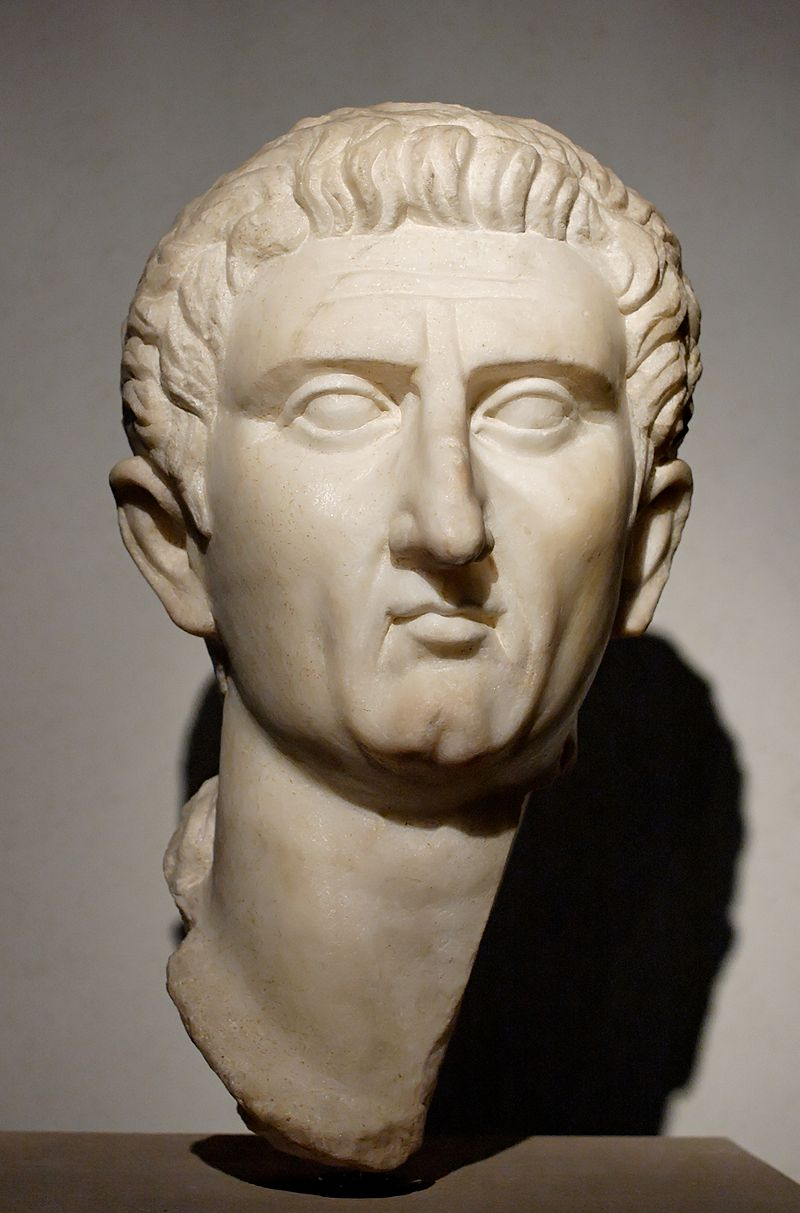
\includegraphics[width=0.17\textwidth]{./Nerva}\label{subfig:Nerva}
	}  
	\subfloat[图拉真]{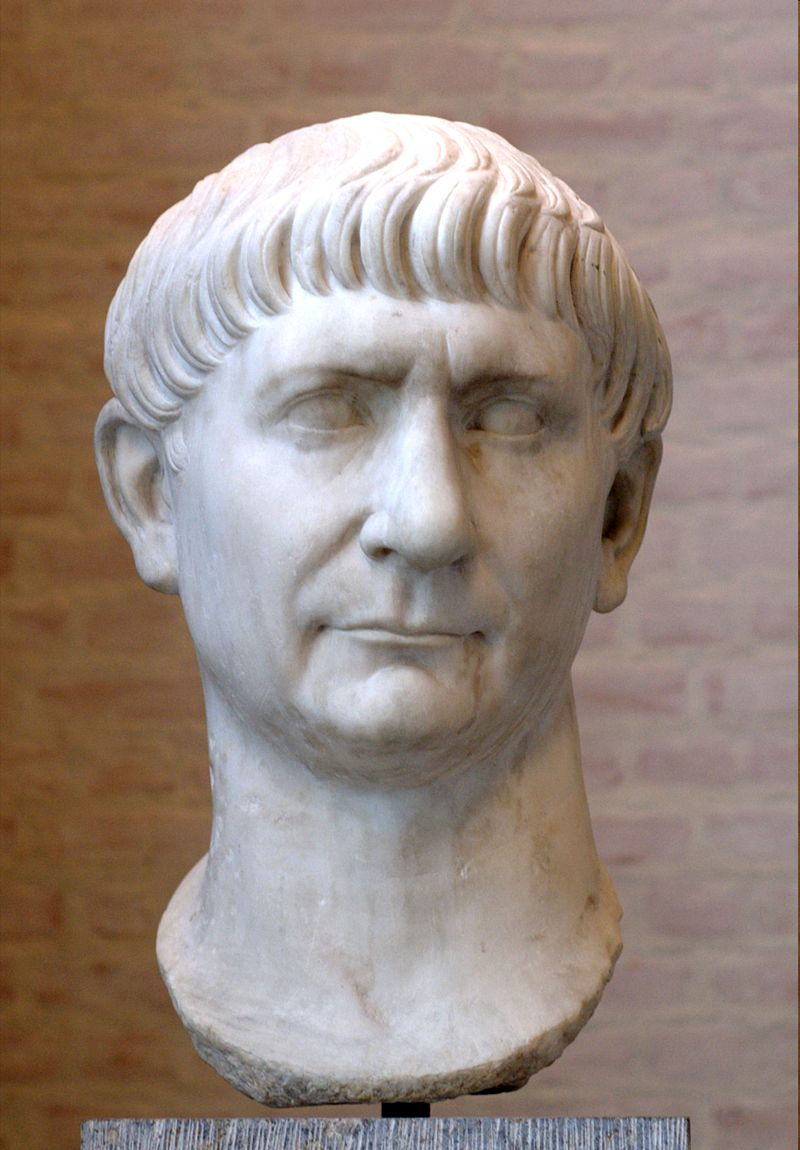
\includegraphics[width=0.17\textwidth]{./Traianus}\label{subfig:Traianus}
	}
	\subfloat[哈德良]{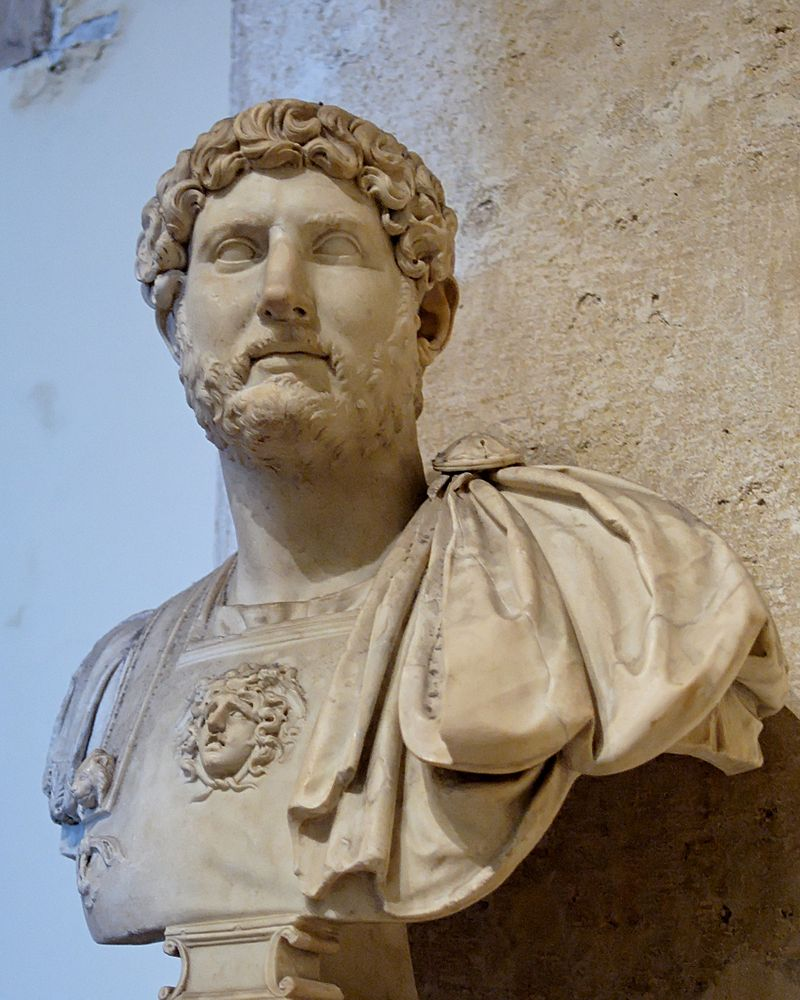
\includegraphics[width=0.17\textwidth]{./Hadrian}\label{subfig:Hadrian}
	}
	\subfloat[安敦尼\ 庇护]{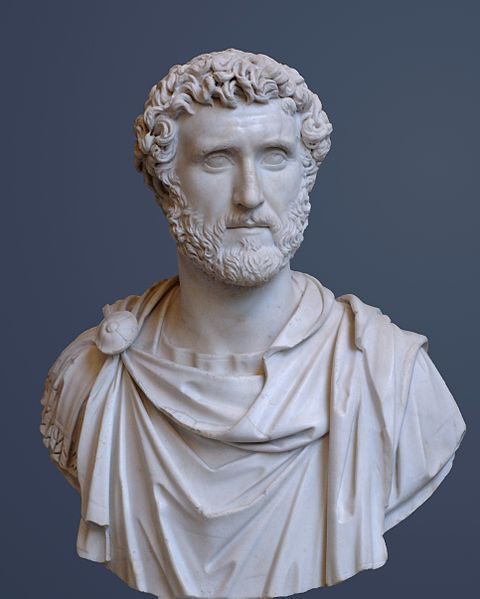
\includegraphics[width=0.17\textwidth]{./Antoninus_Pius}\label{subfig:Antoninus_Pius}
	}
	\subfloat[马可\ 奥勒留]{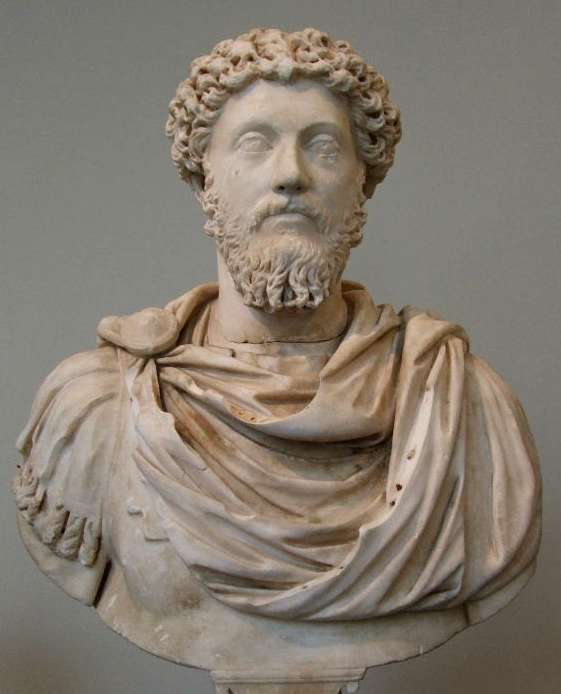
\includegraphics[width=0.17\textwidth]{./Marcus_Aurelius}\label{subfig:Aurelius}
	}    
	\caption{罗马帝国五贤帝.}
	\label{fig:Rome}
\end{figure*}

\cref{fig:Rome} 给出了 5 幅图像,分别是图~\subref*{subfig:Nerva} 涅尓瓦、图~\subref*{subfig:Traianus} 图拉真、
图~\subref*{subfig:Hadrian} 哈德良、图~\subref*{subfig:Antoninus_Pius} 安敦尼\ 庇护 和 图~\subref*{subfig:Aurelius} 马可\ 奥勒留。


\cref{tab:Quantitative} 给出了一个表格的例子。

\begin{table}[htb!]
	\centering
	\setlength{\tabcolsep}{2pt}
	\scriptsize
	\caption{表格示例:定量评价指标比较.}
	\begin{tabular}{lrrrrrrrrrrrrrrr}
		\toprule
		Method & \multicolumn{3}{l}{XXX1} & & \multicolumn{3}{l}{XXX2} & & \multicolumn{3}{l}{XXX3} & & \multicolumn{3}{l}{XXX4} \\ 
		\cmidrule{2-4} \cmidrule{6-8} \cmidrule{10-12} \cmidrule{14-16}
		% \cline{2-4} \cline{6-8} \cline{10-12} \cline{14-16}
		& \multicolumn{1}{l}{指标1} & \multicolumn{1}{l}{指标2} & \multicolumn{1}{l}{指标3} &           & \multicolumn{1}{l}{指标1} & \multicolumn{1}{l}{指标2} & \multicolumn{1}{l}{指标3} &           & \multicolumn{1}{l}{指标1} & \multicolumn{1}{l}{指标2} & \multicolumn{1}{l}{指标3} &           & \multicolumn{1}{l}{指标1} & \multicolumn{1}{l}{指标2} & \multicolumn{1}{l}{指标3} \\
		\midrule          
		Method1 & 1.49                        & 3.20                        & 3.26                        &           & 1.02                        & 3.75                        & 3.44                        &           & 2.80                        & 3.57                        & 3.87                        &           & 2.82                        & 7.51                        & 4.90                        \\
		Method2 & 4.83                        & 8.51                        & 10.90                       &           & 5.64                        & 5.72                        & 7.81                        &           & 3.99                        & 5.68                        & 9.82                        &           & 5.65                        & 19.81                       & 17.75                       \\
		Method3 & 2.64                        & 9.23                        & 10.18                       &           & 5.03                        & 11.11                       & 9.45                        &           & 2.69                        & 8.03                        & 8.80                        &           & 3.92                        & 32.03                       & 21.22                       \\
		Method4 & 8.16                        & 120.54                      & 205.92                      &           & 65.38                       & 74.31                       & 78.27                       &           & 8.39                        & 59.59                       & 83.85                       &           & 10.66                       & 125.06                      & 103.05                      \\
		Method5 & 2.96                        & 8.71                        & 39.94                       &           & 8.83                        & 9.68                        & 11.32                       &           & 3.16                        & 7.01                        & 10.97                       &           & 4.38                        & 23.94                       & 31.47                       \\
		Method6 & 3.91                        & 44.15                       & \textbf{539.44}             & \textbf{} & 18.22                       & 39.38                       & 43.14                       &           & 7.63                        & 51.84                       & 72.81                       &           & \textbf{29.18}              & 309.65                      & \textbf{479.56}             \\
		Method7 & \textbf{19.29}              & \textbf{297.88}             & 533.87                      &           & \textbf{73.70}              & \textbf{623.98}             & \textbf{664.21}             & \textbf{} & \textbf{11.65}              & \textbf{103.58}             & \textbf{149.16}             & \textbf{} & 14.59                       & \textbf{351.90}             & 284.23                      \\
		\bottomrule
	\end{tabular}%
	\label{tab:Quantitative}%
\end{table}%

\subsection*{致谢}
感谢南京航空航天大学戴一冕的模板\href{https://github.com/YimianDai/iNSFC}{iNSFC}。
% {
%   \raggedleft
%   2017 年 2 月 27 日
% }

{
	\raggedleft 
	Yang Luo \\
	2020 年 1 月 29 日\\
}

\NsfcSection{拟采取的研究方案及可行性分析}{(包括研究方法、技术路线、实验手段、关键技术等说明);}

无

\NsfcSection{本项目的特色与创新之处;}{}

无

\NsfcSection{年度研究计划及预期研究结果}{(包括拟组织的重要学术交流活动、国际合作与交流计划等)。}

无

%(二)研究基础与工作条件

\NsfcChapter{(二)研究基础与工作条件}{}

\NsfcSection{研究基础}{(与本项目相关的研究工作积累和已取得的研究工作成绩);}

无

\NsfcSection{工作条件}{(包括已具备的实验条件,尚缺少的实验条件和拟解决的途径,包括利用国家实验室、国家重点实验室和部门重点实验室等研究基地的计划与落实情况);}

无

\NsfcSection{正在承担的与本项目相关的科研项目情况}{(申请人和项目组主要参与者正在承担的与本项目相关的科研项目情况,包括国家自然科学基金的项目和国家其他科技计划项目,要注明项目的名称和编号、经费来源、起止年月、与本项目的关系及负责的内容等);}

无

\NsfcSection{完成国家自然科学基金项目情况}{(对申请人负责的前一个已结题科学基金项目(项目名称及批准号)完成情况、后续研究进展及与本申请项目的关系加以详细说明。另附该已结题项目研究工作总结摘要(限500字)和相关成果的详细目录)。}

无

%(三)其他需要说明的问题

\NsfcChapter{(三)其他需要说明的问题}{}

\NsfcSection{}{申请人同年申请不同类型的国家自然科学基金项目情况(列明同年申请的其他项目的项目类型、项目名称信息,并说明与本项目之间的区别与联系)。}

无

\NsfcSection{}{具有高级专业技术职务(职称)的申请人或者主要参与者是否存在同年申请或者参与申请国家自然科学基金项目的单位不一致的情况;如存在上述情况,列明所涉及人员的姓名,申请或参与申请的其他项目的项目类型、项目名称、单位名称、上述人员在该项目中是申请人还是参与者,并说明单位不一致原因。}

无

\NsfcSection{}{具有高级专业技术职务(职称)的申请人或者主要参与者是否存在与正在承担的国家自然科学基金项目的单位不一致的情况;如存在上述情况,列明所涉及人员的姓名,正在承担项目的批准号、项目类型、项目名称、单位名称、起止年月,并说明单位不一致原因。}

无

\NsfcSection{}{其他。}

无

%%%%%%%%%%%%%%%%%%%%%%%%%%%%%%%%%%%%%%%%%%%%%%%%%

\end{document}
